\chapter{Stabilitásvizsgálat időkéséssel}\label{chap:time_delay_stability}

A modell és a motor paramétereken kívül a rendszer különböző elemeiben megjelenő időkésés 
is hatással van a stabilitásra. Elegendően nagy időkésés mellett nem csak a mozgásra előírt 
feltételek sérülnek, hanem teljesen instabillá válhat a rendszer. Az időkésés hatását analitikusan egyszerűbb 
rendszereknél például a Lambert-féle W-függvény segítségével~\cite{Yi2012, MatrixLambert2007}, 
vagy D-szeparációval lehet vizsgálni. A Lambert-féle W-függvény bonyolultabb rendszereknél nehezen 
vagy egyaltalán nem alkalmazható~\cite{CepedaGomez2015}, így a következő fejezetben a D-szeparáció módszere 
kerül alkalmazásra.

\section{Stabilitás folytonos időben}

Időkésés megjelenhet a rendszer különböző pontjain. A motor kimenetének mérése, az adatáramlás 
a szabályozó részegységei között és a szabályozó jel kiszámítása mind időt vesznek igénybe. 
Ezeknek a hatásoknak az összeségét egy konstans átlag időkésés reprezentálja. A továbbiakban ez a 
paraméter legyen \(\tau_\RM d\).
\begin{figure}[ht]
    \begin{center}
    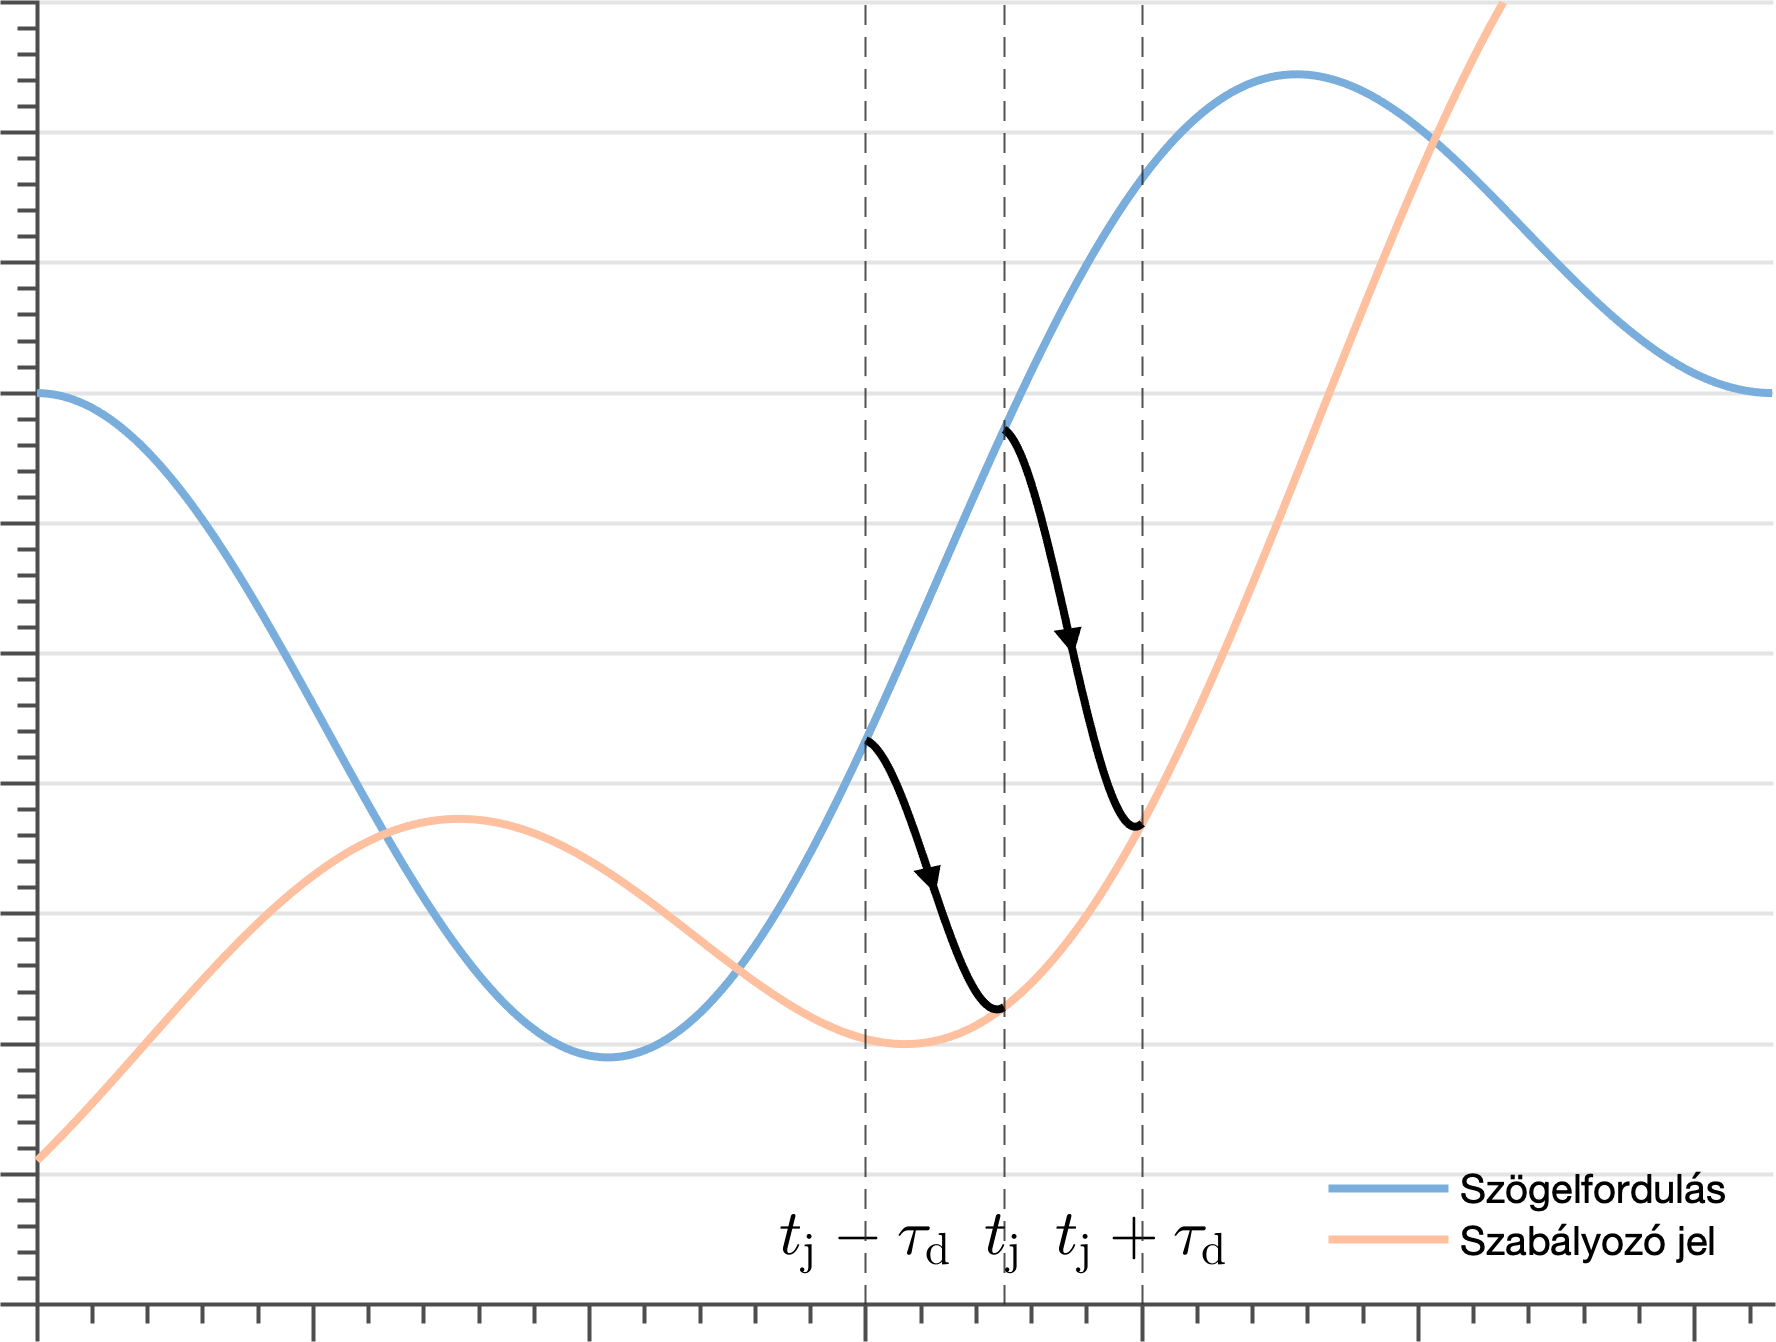
\includegraphics[width=12cm]{images/time_delay_example.png}
    \caption{Reprezentatív ábra az időkésés hatásáról folytonos időben}\label{fig:time_delay_example}
    \end{center}
\end{figure}
A szabályozó jel \(\tau_\RM d\) időegységgel eltolódva jelenik meg a motor bemenetén, ahogy a
~\ref{fig:time_delay_example}. ábra szemlélteti.

A stabilitásvizsgálat az időkéséssel kiegészített szögelfordulás-referencia jel átviteli függvényből 
kiindulva végezhető el. Az időkéséssel kiegészített blokk diagram egyszerűsített alakban 
a~\ref{fig:block_diagram_time_delay}. ábrán látható.
\begin{figure}[ht]
    \begin{center}
    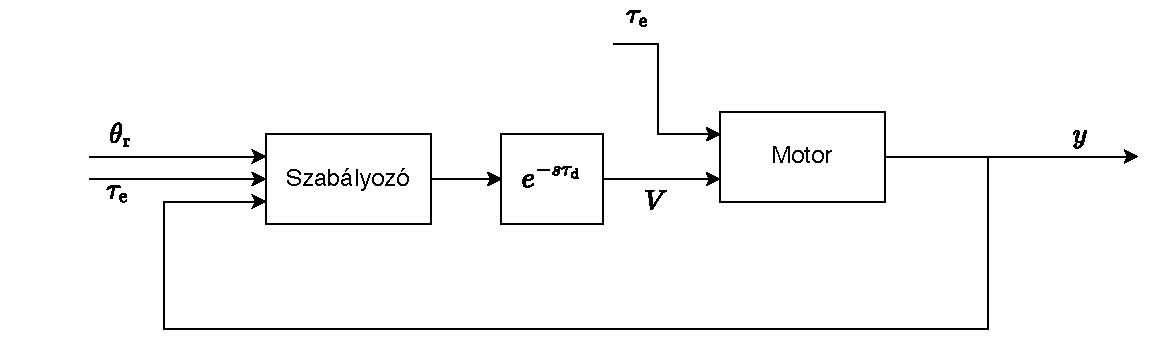
\includegraphics[width=\textwidth]{images/block_diagram_time_delay.pdf}
    \caption{Időkéséssel kiegészített egyszerűsített blokk diagram}\label{fig:block_diagram_time_delay}
    \end{center}
\end{figure}
A motor átviteli függvényei a~\eqref{eq:transfer_function}. egyenletekben szerepelnek. A szabályozó dinamikáját 
az átláthatóság érdekében a következő egyenletek összegzik:
\begin{equation}
    \begin{split}
        \dot{\tilde{\BF \eta}} &= \hat{\BF A} \tilde{\BF \eta} + \hat{\BF B} y + \hat{\BF F}_\RM V V + \hat{\BF F}_\RM \tau \tau_\RM e\,, \\
        \tilde{\BF \eta} &= \tilde{\BF x}_\RM b - \BF K_\RM e y\,, \\
        V &= K_\RM r \theta_\RM r - K_\RM c \tau_\RM e - \BF K \tilde{\BF x}\,,
    \end{split}
\end{equation}
ahol a megfigyelő belső dinamikáját leíró egyenletben megjelenő mátrixok~\eqref{eq:observer_params}-hez hasonlóan:
\begin{align}
    \begin{split}
        \hat{\BF A} &= \BF A_\RM{bb} - \BF K_\RM e \BF A_\RM{ab}\,,\\
        \hat{\BF B} &= \hat{\BF A} \BF K_\RM e + \BF A_\RM {ba} - \BF K_\RM e A_\RM {aa}\,,\\
        \hat{\BF F} &= \BF B_\RM b - \BF K_\RM e B_\RM a\,.
    \end{split}
\end{align}
A kimeneti feszültség egyenletében található becsült állapotvektor kifejezhető a megfigyelő belső állapotával és a mért kimenettel:
\begin{equation}
    \begin{split}
        V &= K_\RM r \theta_\RM r - K_\RM c \tau_\RM e - (K_a + \BF K_\RM b \BF K_\RM e) y - \BF K_\RM b \tilde{\BF \eta}\,,
    \end{split}
\end{equation}
behelyettesítve a megfigyelő dinamikai egyenletébe:
\begin{align}\label{eq:observer_transfer_transformed}
    \begin{split}
        \dot{\tilde{\BF \eta}} &= \hat{\BF A} \tilde{\BF \eta} + 
        \hat{\BF B} y + 
        \hat{\BF F}_\RM V\left[K_\RM r \theta_\RM r - K_\RM c \tau_\RM e - (K_a + \BF K_\RM b \BF K_\RM e) y - \BF K_\RM b \tilde{\BF \eta}\right] + 
        \hat{\BF F}_\RM \tau \tau_\RM e \\
        &= (\hat{\BF A} - \hat{\BF F}_\RM V \BF K_\RM b)\tilde{\BF \eta} + 
        [\hat{\BF B} - \hat{\BF F}_\RM V (K_\RM a + \BF K_\RM b \BF K_\RM e)]y + 
        \hat{\BF F}_\RM V K_\RM r \theta_\RM r + 
        (\hat{\BF F}_\RM \tau - \hat{\BF F}_\RM V K_\RM c) \tau_\RM e\,.
    \end{split}
\end{align}
A szabályozó dinamikája ez alapján kifejezhető egy új állapottér modell formájában:
\begin{align}\label{eq:controller_state_space}
    \begin{split}
        \dot{\tilde{\BF \eta}} &= \tilde{\BF A}\tilde{\BF \eta} + 
        \tilde{\BF B}_\RM y y + 
        \tilde{\BF B}_\RM r \theta_\RM r +
        \tilde{\BF B}_\RM \tau \tau\RM e\,, \\
        V &= \tilde{\BF C}\tilde{\BF \eta} + 
        \tilde{\BF D}_\RM y y + 
        \tilde{\BF D}_\RM r \theta_\RM r + 
        \tilde{\BF D}_\RM \tau \tau_\RM e\,,
    \end{split}
\end{align}
ahol a mátrix paraméterek~\eqref{eq:observer_transfer_transformed} szerint:
\begin{align}
    \begin{split}
        \tilde{\BF A} &= \hat{\BF A} - \hat{\BF F}_\RM V \BF K_\RM b\,,\\
        \tilde{\BF B}_\RM y &= \hat{\BF B} - \hat{\BF F}_\RM V (K_\RM a + \BF K_\RM b \BF K_\RM e)\,,\\
        \tilde{\BF B}_\RM r &= \hat{\BF F}_\RM V K_\RM r\,, \\
        \tilde{\BF B}_\RM \tau &= \hat{\BF F}_\RM \tau - \hat{\BF F}_\RM V K_\RM c\,, \\
        \tilde{\BF C} &= -\BF K_\RM b\,, \\
        \tilde{\BF D}_\RM y &= -(K_\RM a + \BF K_\RM b \BF K_\RM e)\,, \\
        \tilde{\BF D}_\RM r &= K_\RM r\,, \\
        \tilde{\BF D}_\RM \tau &= -K_\RM c\,.
    \end{split}
\end{align}
A szabályozó és a motor állapottér egyenletei időkéséssel kiegészítve a következő átviteli 
függvénnyel írhatók le:
\begin{align}
    \begin{split}
        y = \left(C^\RM V_\RM r \theta_\RM r + 
        C^\RM V_\RM \tau \tau_\RM e +
        C^\RM V_\RM y y\right)M^\RM y_\RM V e^{-s\tau_\RM d} +
        M^\RM y_\RM\tau \tau_\RM e\,,
    \end{split}
\end{align}
ahol a \(C^\RM n_\RM m\) és \(M^\RM n_\RM m\) a szabályozó és a motor átviteli függvényei adott 
bemenetekre és kimenetekre. A felső index jelöli a kimenetet, az alsó index pedig a bemenetet.
Az átviteli egyenlet zárt körben:
\begin{align}
    \begin{split}
        y = \frac{1}{1 - M^\RM y_\RM V C^\RM V_\RM y e^{-s\tau_\RM d}}
        \left[
            M^\RM y_\RM V C^\RM V_\RM r \theta_\RM r e^{-s\tau_\RM d} + 
            \left(M^\RM y_\RM\tau + M^\RM y_\RM V C^\RM V_\RM \tau e^{-s\tau_\RM d}\right) \tau_\RM e
        \right]
    \end{split}
\end{align}
alakban írható le. A motor és a szabályozó átviteli függvényei bemenettől és kimenettől 
függetlenül ugyanazokkal a pólusokkal rendelkeznek, így mindkét bemenetre ugyanazok a stabilitási 
feltételek érvényesek. Az átviteli függvény pólusait a következő egyenlet megoldásai adják:
\begin{align}\label{eq:delay_characteristic}
    \begin{split}
        &s^5 + 
        \left(c_{41} + c_{42}\frac{B_\RM e}{M_\RM e}\right)s^4 +
        \left(c_{31} + c_{32}\frac{B_\RM e}{M_\RM e} + c_{33}\frac{K_\RM e}{M_\RM e}\right)s^3 + \\
        &\left[c_{21} + c_{22}\frac{B_\RM e}{M_\RM e} + c_{23}\frac{K_\RM e}{M_\RM e} + \left(
        c_{24} + c_{25}\frac{B_\RM e}{M_\RM e} + c_{26}\frac{K_\RM e}{M_\RM e}\right)e^{-s\tau_\RM d}\right]s^2 + \\
        &\left[c_{11} + c_{12}\frac{B_\RM e}{M_\RM e} + c_{13}\frac{K_\RM e}{M_\RM e} + \left(
        c_{14} + c_{15}\frac{B_\RM e}{M_\RM e} + c_{16}\frac{K_\RM e}{M_\RM e}\right)e^{-s\tau_\RM d}\right]s + 
        c_0 \frac{K_\RM e}{M_\RM e} = 0\,,
    \end{split}
\end{align}
ahol az együtthatókat a ... táblázat tartalmazza. D-szeparációt alkalmazva az egyenlet valós és 
képzetes részei:
\begin{align}\label{eq:delay_complex_separation}
    \begin{split}
        a_4\omega^4-(a_{21} + a_{22}\cos{\omega\tau_\RM d})\omega^2+a_{12}\omega\sin{\omega\tau_\RM d} + a_0\cos{\omega\tau_\RM d} &= 0 \\
        \omega^5 -a_3\omega^3 + a_{22}\omega^2\sin{\omega\tau_\RM d} + (a_{11} + a_{12}\cos{\omega\tau_\RM d})\omega - a_0\sin{\omega\tau_\RM d}  &= 0 \,,
    \end{split}
\end{align}
melyek \(s=jw\) behelyettesítés után adódnak. Az új együtthatók~\eqref{eq:delay_characteristic} alapján:
\begin{align}
    \begin{split}
        a_4 &= c_{41} + c_{42}\frac{B_\RM e}{M_\RM e}\\ 
        a_3 &= c_{31} + c_{32}\frac{B_\RM e}{M_\RM e} + c_{33}\frac{K_\RM e}{M_\RM e}\\ 
        a_{21} &= c_{21} + c_{22}\frac{B_\RM e}{M_\RM e} + c_{23}\frac{K_\RM e}{M_\RM e}\\ 
        a_{22} &= c_{24} + c_{25}\frac{B_\RM e}{M_\RM e} + c_{26}\frac{K_\RM e}{M_\RM e}\\ 
        a_{11} &= c_{11} + c_{12}\frac{B_\RM e}{M_\RM e} + c_{13}\frac{K_\RM e}{M_\RM e}\\ 
        a_{12} &= c_{14} + c_{15}\frac{B_\RM e}{M_\RM e} + c_{16}\frac{K_\RM e}{M_\RM e}\\ 
        a_0 &= c_0 \frac{K_\RM e}{M_\RM e}\,.
    \end{split}
\end{align}
A~\eqref{eq:delay_complex_separation}-ben szereplő egyenletrendszert megoldva \(\frac{B_\RM e}{M_\RM e}\)
és \(\frac{K_\RM e}{M_\RM e}\) kifejezésekre egy paraméteres görbe adódik. 
A független paraméter \(\omega\) a stabilitás határán fellépő csillapítatlan rezgés frekvenciájával
arányos. A görbe minden pontjához egy tisztán képzetes póluspár vagy nulla kapcsolódik. 
A nulla megoldások a \(\frac{K_\RM e}{M_\RM e} = 0\) egyenesen helyezkednek el. 
A kapott görbét a~\ref{tab:delay_stab_params}. táblázat paramétereit behelyettesítve 
a~\ref{fig:time_delay_stab_map}. ábra mutatja. A kontúrvonalakon szereplő értékek \(\tau_\RM d\)
időkésés különböző értékeit jelölik szekundumban kifejezve.

\begin{table}[ht]
    \small\centering
    \caption{A folytonos idejű stabilitásvizsgálatnál alkalmazott paraméterek}\label{tab:delay_stab_params}
    \tabcolsep=1pt
    \begin{tabular}{l>{~}l>{\quad}rl}
        \toprule
        \multicolumn{2}{c}{Szimbólum és paraméter név} & \multicolumn{2}{c}{Érték} \\ \midrule
        \(J\) & Motor tehetetlensége & 0.01 & \(\RM{kg\cdot m^2}\) \\
        \(K_\RM m\) & Motor nyomatékállandója & 0.01 & \(\RM{Nm\cdot A^{-1}}\) \\
        \(B_\RM m\) & Motor modell viszkózus csillapítása & 0.1 & \(\RM{kg\cdot m^2\cdot s^{-1}}\) \\
        \(L\) & Motor induktivitása & 0.2 & H \\
        \(R\) & Motor ellenállása & 1 & \(\Omega\) \\
        \(p\) & További pólusok & -15 & \(\RM{rad \cdot s^{-1}}\) \\
        \(K_\RM c\) & Nyomaték kompenzációs együttható & -50 & \(\RM{V \cdot N^{-1} m^{-1}}\) \\
        \bottomrule
    \end{tabular}
\end{table}

\begin{figure}[ht]
    \begin{center}
    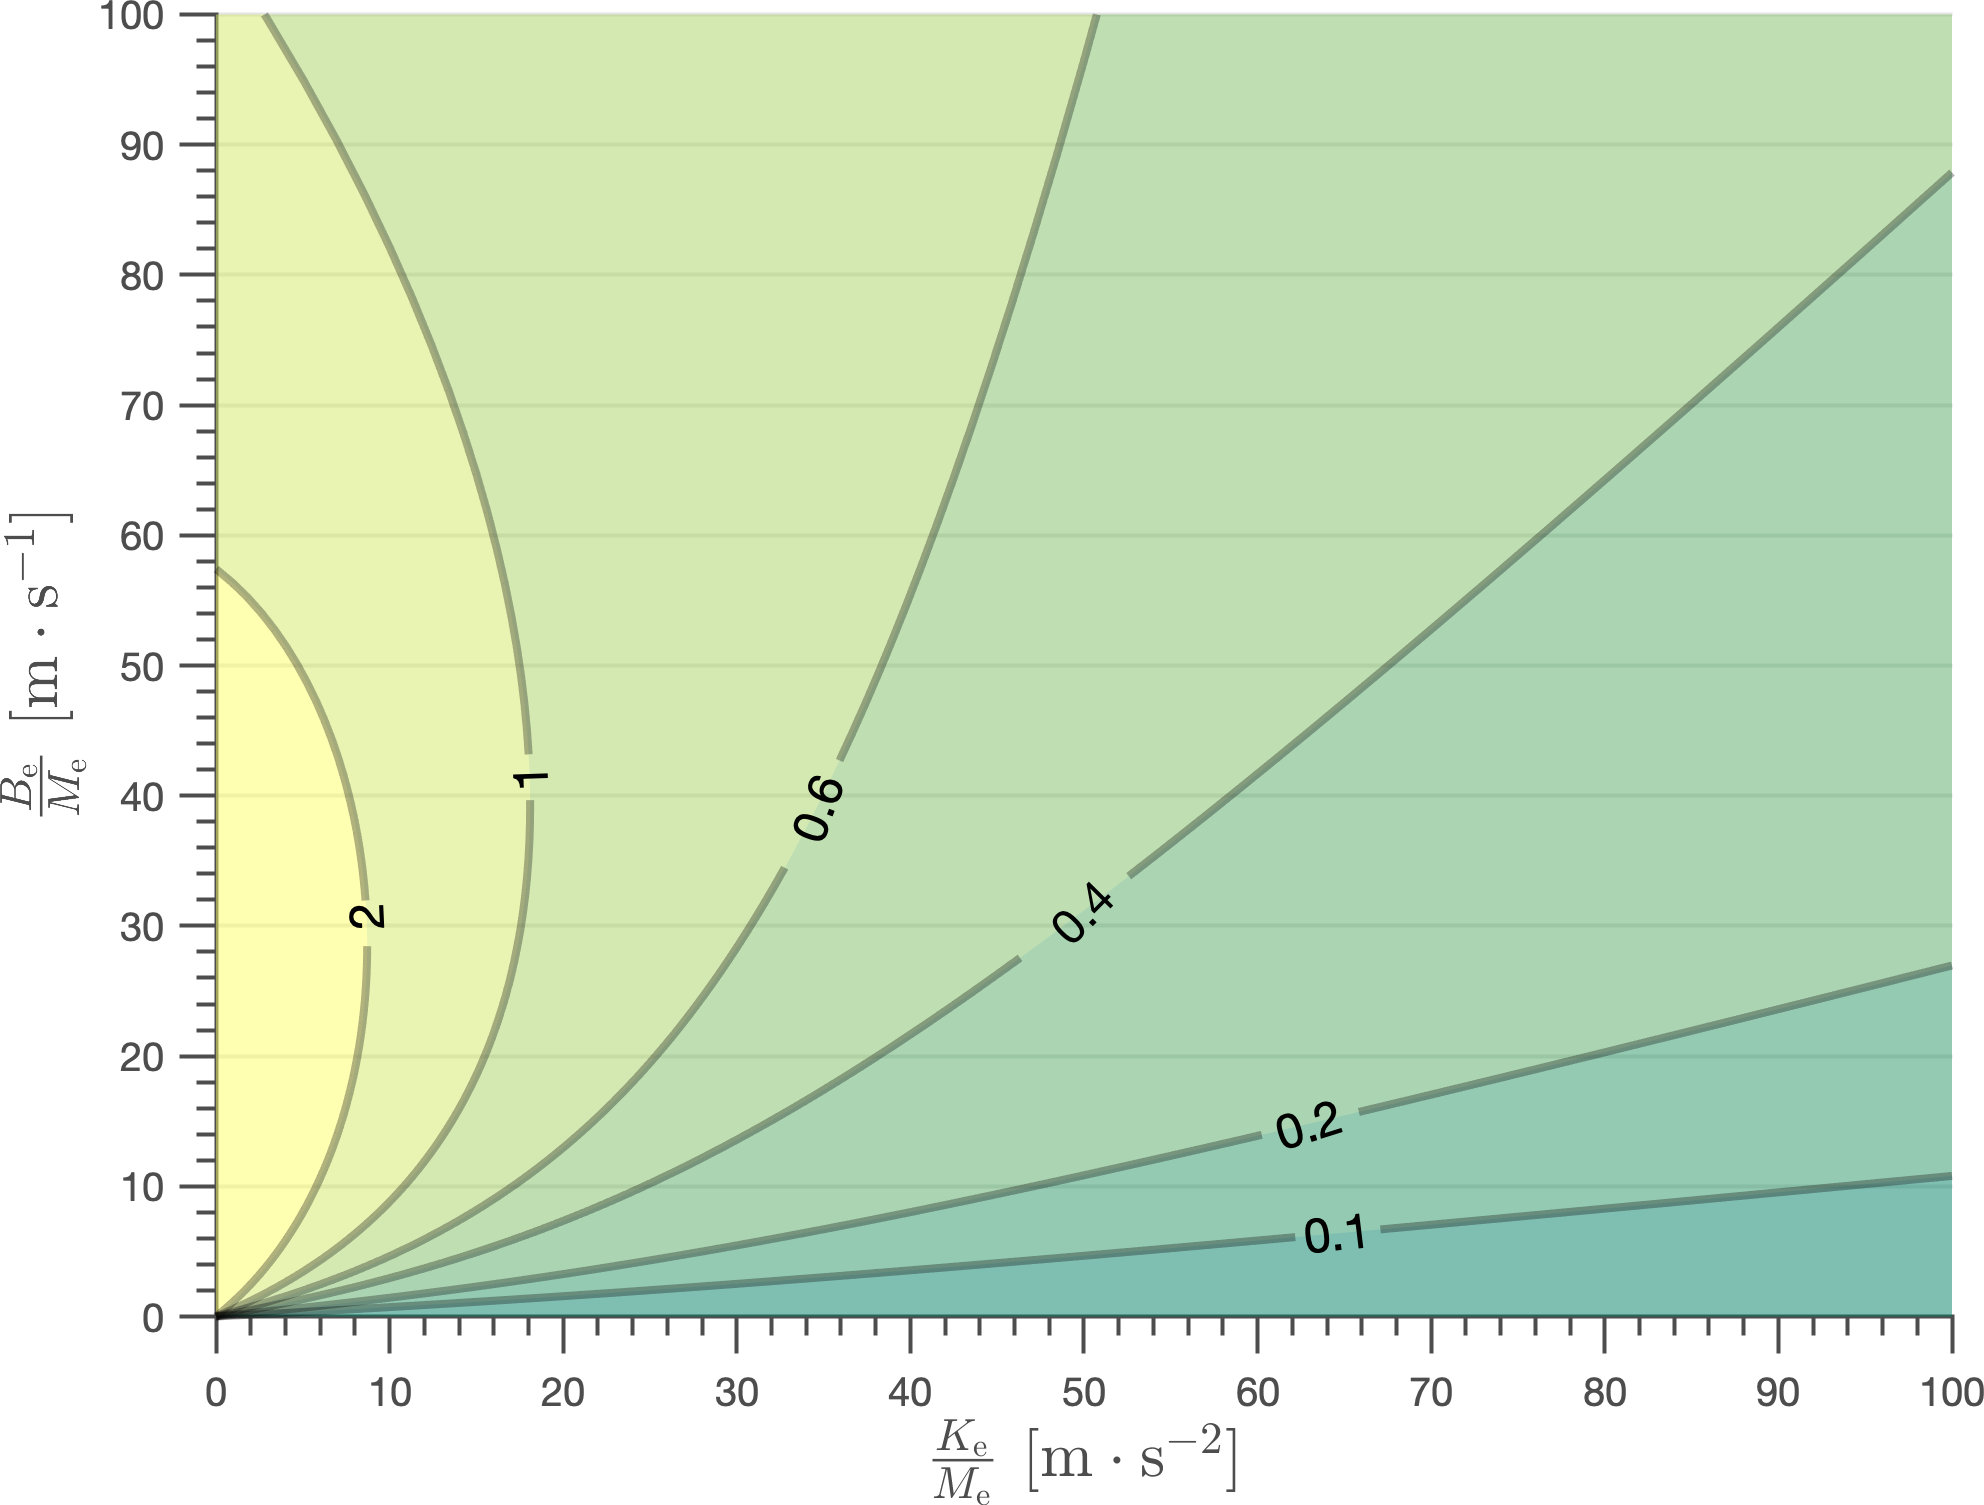
\includegraphics[width=\textwidth]{images/time_delay_stab_map.png}
    \caption{Folytonos idejű stabilitástérkép}\label{fig:time_delay_stab_map}
    \end{center}
\end{figure}

Időkésés nélkül a görbe pontjai a \(\frac{B_\RM e}{M_\RM e} = 0\) egyenesen maradnak.
A behatárolt stabilitástartomány éppen megegyezik a Routh--Hurwitz kritérium által 
kapott tartománnyal, tehát:
\begin{equation}
    M_\RM e > 0,~~B_\RM e > 0,~~K_\RM e > 0.
\end{equation}
Az időkésés növekedésével egyre szűkül a stabil tartomány, egy kritikus érték alatt azonban
csak \(\frac{K_\RM e}{M_\RM e}\) kifejezésre adódik maximum, \(\frac{B_\RM e}{M_\RM e}\)
tetszőleges pozitív értéket felvehet. A kritikus időkésés felett egy véges területet határolnak be 
a görbe \(\omega > 0\) és \(\omega = 0\) szegmensei. 

\section{Stabilitás diszkrét időben}
A folytonos időben végzett stabilitásvizsgálat alapján belátható, hogy az 
időkésés korlátozza az impedancia modell által előírható paramétereket.
A valós rendszerben egy digitális feldolgozóegység végzi el a szabályozó jel
meghatározásához szükséges számításokat, közel állandó időnként. Két ilyen 
ciklus között a szabályozó jel állandó marad. Ezeket figyelembe véve a 
folytonos időben végzett stabilitásvizsgálat eredménye tovább pontosítható.
\begin{figure}[ht]
    \begin{center}
    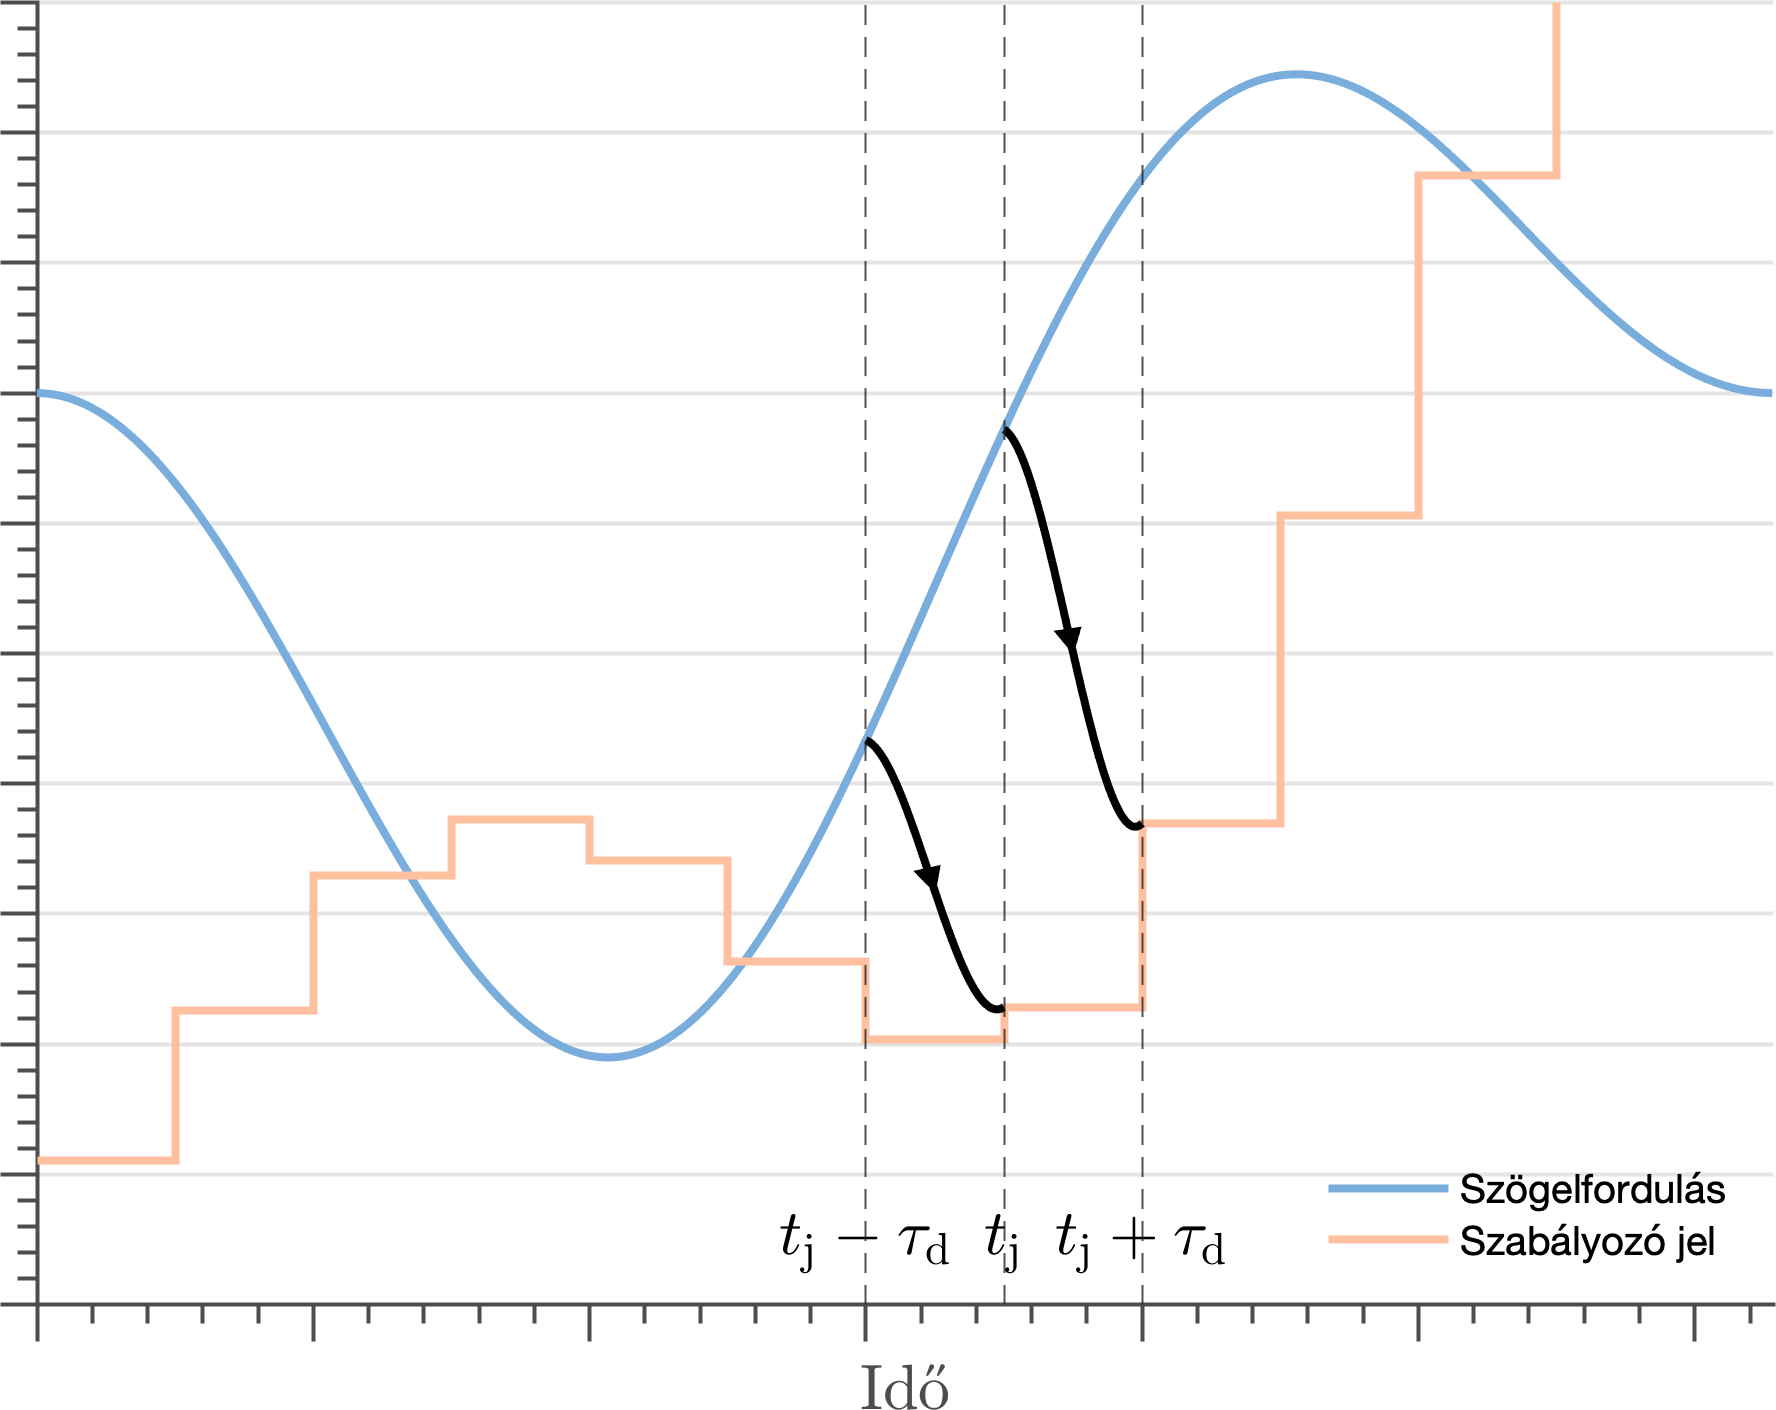
\includegraphics[width=12cm]{images/time_delay_example_discrete.png}
    \caption{Reprezentatív ábra az időkésés hatásáról diszkrét időben}\label{fig:time_delay_example_discrete}
    \end{center}
\end{figure}

A mért szögelfordulás és a diszkrét idejű szabályozó jel kapcsolatát szemlélteti a~\ref{fig:time_delay_example_discrete}. ábra.
Két mintavételezési pont között a szabályozó jel állandó marad (zero-order hold). A mért szögelfordulás érték 
feldolgozása után az új szabályozó jel mindig egy mintavételezési periódussal később jelenik meg a motor bemenetén.
A továbbiakban feltételezett, hogy a jelfeldolgozáshoz szükséges időn kívül minden egyéb késés elhanyagolható, 
így a mintavételezési periódus megegyezik a korábban bevezetett \(\tau_\RM d\) időkéséssel. Legyen \(C(t-\tau(t))\) 
a szabályozó jel időfüggvénye. Ebben az alakban a mintavételezési pontok között konstans kimenet feltétele, hogy 
az időkésés maga (\(\tau(t)\)) egy periodikus fűrész jelet kövessen, ahogy a~\ref{fig:time_delay_example_zoh}. ábra is mutatja.

\begin{figure}[ht]
    \begin{center}
    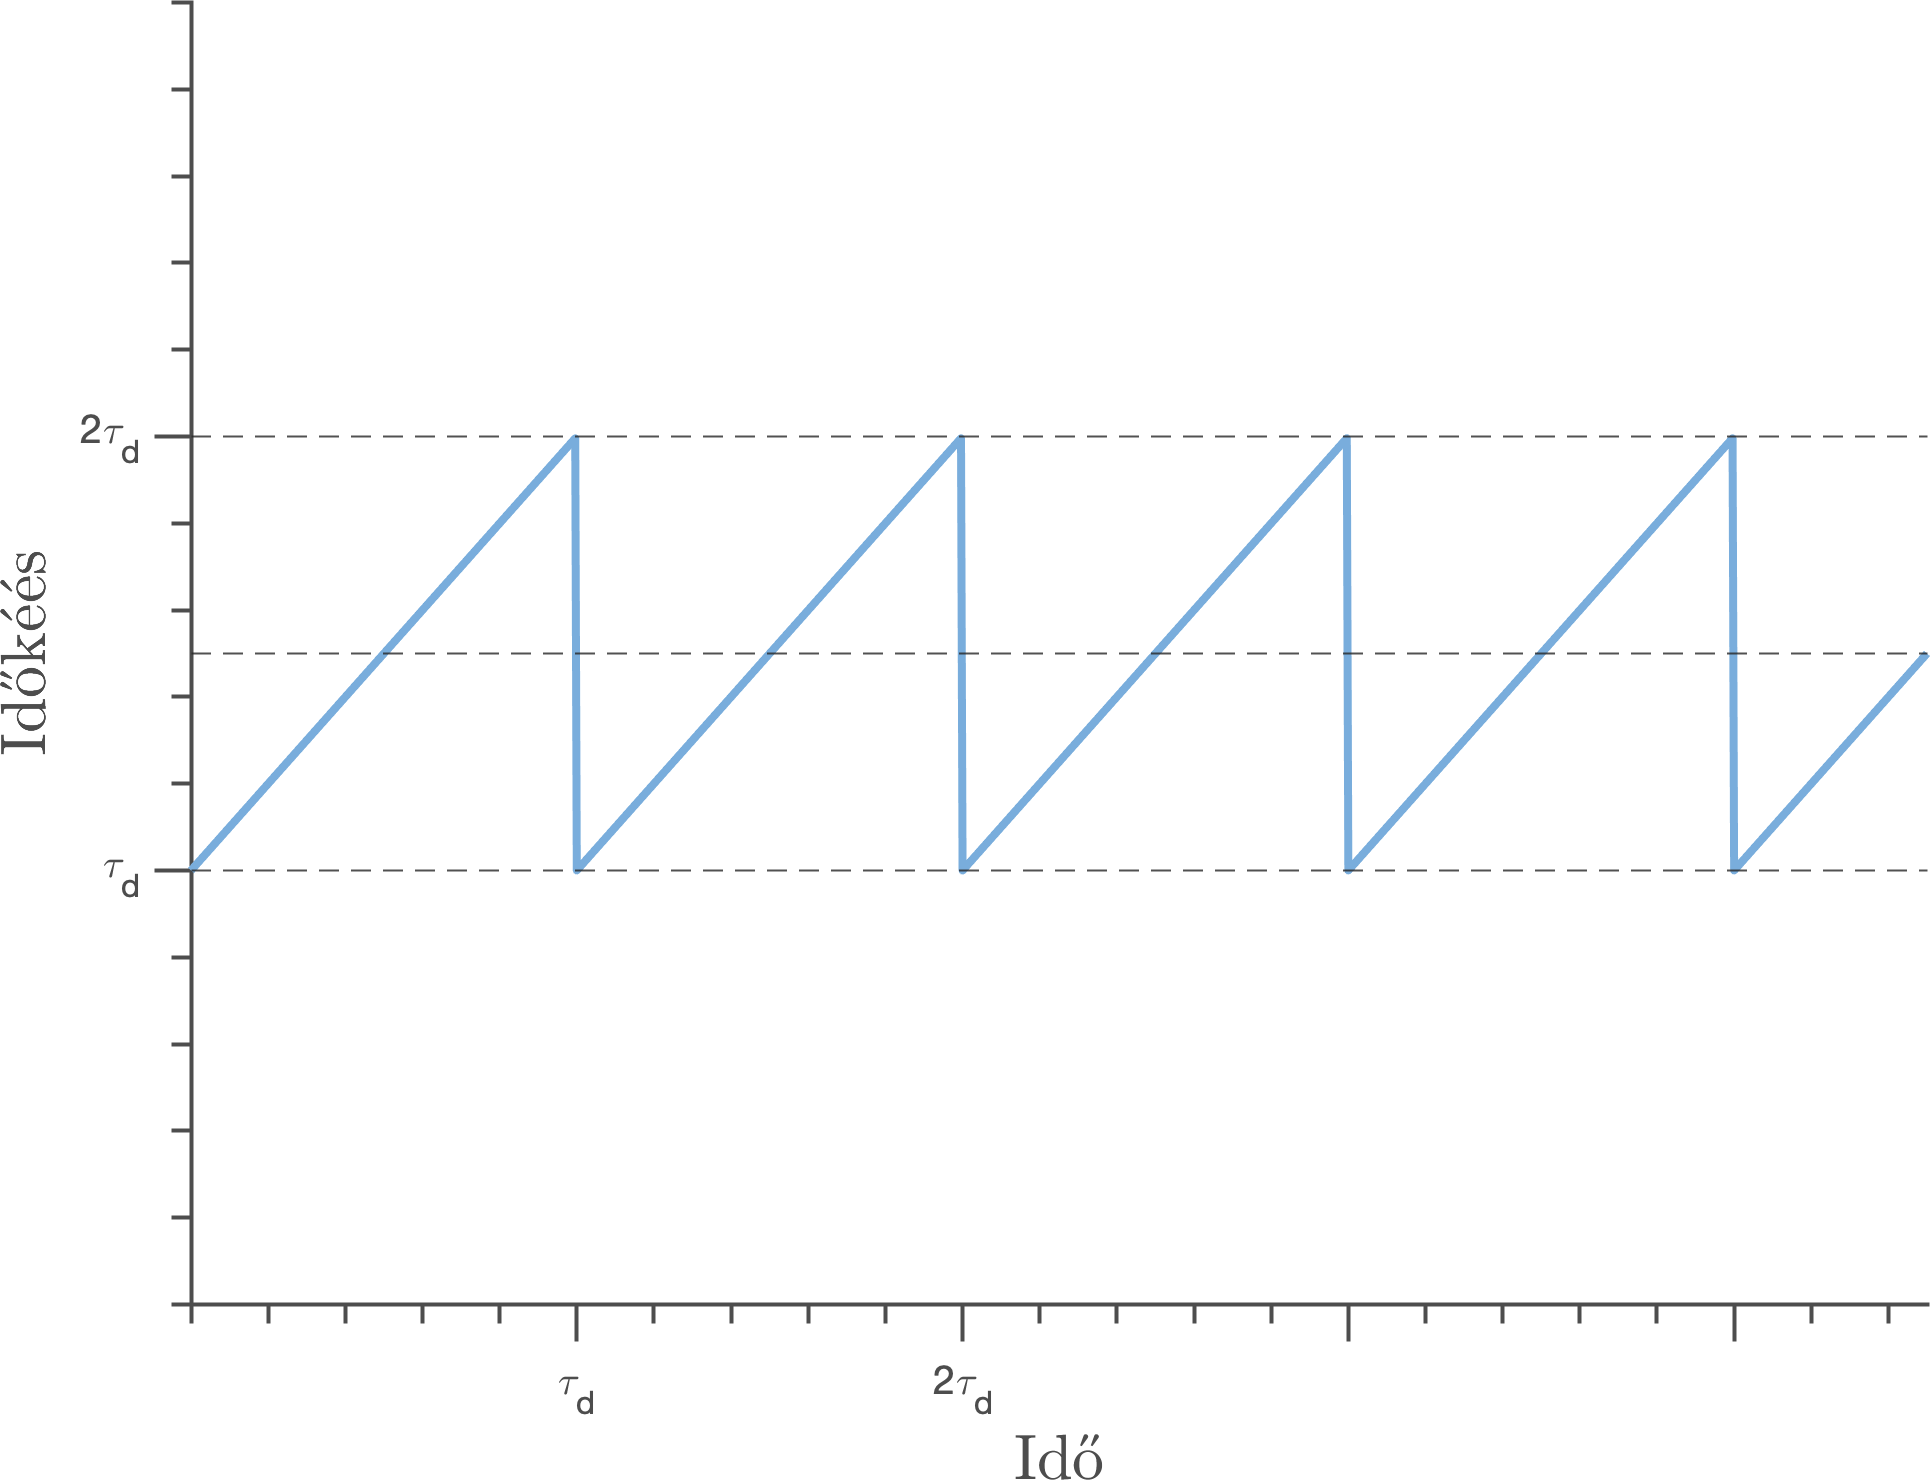
\includegraphics[width=12cm]{images/delay_zoh_example_discrete.png}
    \caption{Az időkésés periodikus függvénye}\label{fig:time_delay_example_zoh}
    \end{center}
\end{figure}

A diszkrét idejű stabilitásvizsgálathoz először diszkretizálni kell a szabályozó folytonos idejű állapottér modelljét.
Ehhez legyen a kiindulási alap a~\eqref{eq:controller_state_space}. egyenletek által definiált modell.
Beszorozva mindkét oldalt \(e^{-\tilde {\BF A} t}\)-vel:
\begin{align}
    \begin{split}
        e^{-\tilde {\BF A} t}\dot\tilde{\BF \eta}(t) &= e^{-\tilde {\BF A} t}\tilde {\BF A} \tilde{\BF \eta}(t) +
        e^{-\tilde {\BF A} t}\left[\tilde{\BF B}_\RM y y(t) + 
        \tilde{\BF B}_\RM r \theta_\RM r(t) +
        \tilde{\BF B}_\RM \tau \tau_\RM e(t)\right] \\
        \frac{\RM d}{\RM d t}\left(e^{-\tilde {\BF A} t}\tilde{\BF \eta}(t)\right) &= e^{-\tilde {\BF A} t}\left[\tilde{\BF B}_\RM y y(t) + 
        \tilde{\BF B}_\RM r \theta_\RM r(t) +
        \tilde{\BF B}_\RM \tau \tau_\RM e(t)\right]\,, 
    \end{split}        
\end{align}
a kapott egyenletet integrálva:
\begin{align}\label{eq:controller_state_integral}
    \begin{split}
        e^{-\tilde {\BF A} t}\tilde{\BF \eta}(t) - e^0 \tilde{\BF \eta}(0) &= \int_{0}^{t} e^{-\tilde {\BF A} t'}\left[\tilde{\BF B}_\RM y y(t') + 
        \tilde{\BF B}_\RM r \theta_\RM r(t') +
        \tilde{\BF B}_\RM \tau \tau_\RM e(t')\right] \RM dt' \\
        \tilde{\BF \eta}(t) &= e^{\tilde {\BF A} t}\tilde{\BF \eta}(0) + \int_{0}^{t} e^{\tilde {\BF A} (t-t')}\left[\tilde{\BF B}_\RM y y(t') + 
        \tilde{\BF B}_\RM r \theta_\RM r(t') +
        \tilde{\BF B}_\RM \tau \tau_\RM e(\tau)\right] \RM dt'\,.
    \end{split}        
\end{align}
A mintavételezési periódus alatt a szabályozó összes bemenete konstans marad, így a bemenetek az 
integrálon kívülre helyezhetők. Legyen \(\tilde{\BF \eta}[k] := \tilde{\BF \eta}(k\tau_\RM d)\) a 
a szabályázó belső állapota a \(k\)-adik diszkrét időlépésnél. Ezzel a~\eqref{eq:controller_state_integral}. 
egyenlet a \(k\)-adik és a (\(k+1\))-edik lépéseknél:
\begin{align}
    \begin{split}
        \tilde{\BF \eta}[k] &= e^{\tilde {\BF A} k\tau_\RM d}\tilde{\BF \eta}(0) + \int_{0}^{k\tau_\RM d} e^{\tilde {\BF A} (k\tau_\RM d-t')}\left[\tilde{\BF B}_\RM y y(t') + 
        \tilde{\BF B}_\RM r \theta_\RM r(t') +
        \tilde{\BF B}_\RM \tau \tau_\RM e(t')\right]\RM dt' \\
        \tilde{\BF \eta}[k+1] &= e^{\tilde {\BF A}\tau_\RM d}\tilde{\BF \eta}[k] + \int_{k\tau_\RM d}^{(k+1)\tau_\RM d} e^{\tilde {\BF A} (k\tau_\RM d + \tau_\RM d-t')}\left[\tilde{\BF B}_\RM y y(t') + 
        \tilde{\BF B}_\RM r \theta_\RM r(t') +
        \tilde{\BF B}_\RM \tau \tau_\RM e(t')\right] \RM dt' \\
        \tilde{\BF \eta}[k+1] &= e^{\tilde {\BF A}\tau_\RM d}\tilde{\BF \eta}[k] + \int_{k\tau_\RM d}^{(k+1)\tau_\RM d} e^{\tilde {\BF A} (k\tau_\RM d + \tau_\RM d-t')}\RM dt'\left[\tilde{\BF B}_\RM y y[k] + 
        \tilde{\BF B}_\RM r \theta_\RM r[k] +
        \tilde{\BF B}_\RM \tau \tau_\RM e[k]\right] \\
        \tilde{\BF \eta}[k+1] &= e^{\tilde {\BF A}\tau_\RM d}\tilde{\BF \eta}[k] + \tilde{\BF A}^{-1}\left(e^{\tilde {\BF A}\tau_\RM d}-\BF I\right)\left[\tilde{\BF B}_\RM y y[k] + 
        \tilde{\BF B}_\RM r \theta_\RM r[k] +
        \tilde{\BF B}_\RM \tau \tau_\RM e[k]\right]\,.
    \end{split}        
\end{align}
Tehát a diszkrét idejű szabályozó állapotér modelljét leírő mátrixok:
\begin{align}\label{eq:discrete_controller_matrices}
    \begin{split}
        \tilde{\BF A}_\RM d &= e^{\tilde {\BF A}\tau_\RM d} \\
        \tilde{\BF B}_\RM d &= \tilde{\BF A}^{-1}\left(e^{\tilde {\BF A}\tau_\RM d}-\BF I\right)\left[\tilde{\BF B}_\RM y~~\tilde{\BF B}_\RM r~~\tilde{\BF B}_\RM \tau\right] \\
        \tilde{\BF C}_\RM d &= \tilde{\BF C} \\
        \tilde{\BF D}_\RM d &= \tilde{\BF D} \,,
    \end{split}        
\end{align}
ahol a mátrix exponenciális kifejezés szükség esetén például Taylor polinommal közelíthető. A további számítások ezt 
a pontos alakot használják.

Következő lépésként a zárt kör dinamkáját is ki kell fejezni a diszkrét időlépések függvényeként. 
A szabályozónál alkalmazott levezetéshez hasonlóan~\eqref{eq:state_space}-ban szereplő mátrixok alapján:
\begin{align}\label{eq:discrete_motor_state}
    \begin{split}    
        \BF x[k+1] &= e^{\BF A \tau_\RM d}\BF x[k] + 
        \BF A^{-1}\left(e^{\BF A \tau_\RM d} - \BF I\right)\BF B_\RM V V[k-1] + 
        \int_{k\tau_\RM d}^{(k+1)\tau_\RM d} e^{\BF A (k\tau_\RM d + \tau_\RM d-t')}\BF B_\RM \tau \tau_\RM e(t')~\RM dt'\\
        y[k] &= \BF C \BF x[k]\,.
    \end{split}        
\end{align}
ahol megjelenik \(V[k-1]\) a szabályozó jel egy egész mintavételezési periódussal késleltetett értéke. 
Legyenek a diszkretizált motor modell új paraméterei:
\begin{align}\label{eq:discrete_motor_matrices}
    \begin{split}
        \BF A_\RM d &= e^{\BF A\tau_\RM d} \\
        \BF B_\RM d &= \BF A^{-1}\left(e^{\BF A\tau_\RM d}-\BF I\right)\BF B_\RM V \\
        \BF C_\RM d &= \BF C \\
        \BF D_\RM d &= \BF D \,.
    \end{split}        
\end{align}

A stabilitásvizsgálathoz a bemenet zérus. A következőkben a zárt kör teljes dinamikájának levezetése 
következik zérus bemenettel. A~\eqref{eq:discrete_motor_state} állapotegyenletbe behelyettesítve a 
szabályozó késleltetett kimenetét:
\begin{align}
    \begin{split}
    \BF x[k+1] &= \BF A_\RM d x[k] + 
    \BF B_\RM d \left(\tilde{\BF C}_\RM d \tilde{\BF \eta}[k-1] + 
    \tilde{\BF D}_\RM {d,y} y[k-1]\right)\,'
    \end{split}        
\end{align}
Felhasználva \(\tilde{\BF \eta}\) és a paraméterek definícióját:
\begin{align}\label{eq:discrete_motor_state_closed}
    \begin{split}
        \BF x[k+1] &= \BF A_\RM d x[k] - 
        \BF B_\RM d \BF K_\RM a y[k-1] - 
        \BF B_\RM d \BF K_\RM b \tilde{\BF x}_\RM b[k-1] \\
        &= \BF A_\RM d x[k] - 
        \BF B_\RM d \BF K \BF x[k-1] +
        \BF B_\RM d \BF K_\RM b \BF e[k-1]\,.
    \end{split}        
\end{align}
A becsült állapot hibájának differencia egyenletei pedig:
\begin{align}
    \begin{split}
        \BF e[k+1] &= \BF x_\RM b[k+1] - \tilde{\BF x}_\RM b[k+1] \\
        &= \BF E_{\RM{xa},k}\BF x_\RM a[k] + 
        \BF E_{\RM{xb},k}\BF x_\RM b[k] + 
        \BF E_{\RM x,k-1}\BF x[k-1] + 
        \BF E_{\RM e,k}\BF e[k] + 
        \BF E_{\RM e,k-1}\BF e[k-1]
        \,,
    \end{split}        
\end{align}
ahol a mátrix együtthatók:
\begin{align}
    \begin{split}
        \BF E_{\RM{xa},k} &= \BF A_\RM{d,ba} + 
        \tilde{\BF A}_\RM d \BF K_\RM e -
        \BF K_\RM e \BF A_\RM{d,aa} \\
        \BF E_{\RM{xb},k} &= \BF A_\RM{d,bb} + 
        \tilde{\BF A}_\RM d -
        \BF K_\RM e \BF A_\RM{d,ab} \\
        \BF E_{\RM x,k-1} &= -(\BF B_\RM{d,b} -
        \BF K_\RM e \BF B_\RM{d,a})\RM K \\
        \BF E_{\RM e,k} &= \tilde{\BF A}_\RM d \\
        \BF E_{\RM e,k-1} &= (\BF B_\RM{d,b} -
        \BF K_\RM e \BF B_\RM{d,a})\RM K_\RM b\,.
    \end{split}        
\end{align}
A~\eqref{eq:pos_control_dynamics} egyenlethez hasonlóan a 
teljes rendszer belső állapotának dinamikája:
\begin{align}
    \begin{split}
        \begin{bmatrix}
        \BF x[k] \\
        \BF e[k] \\
        \BF x[k+1] \\ 
        \BF e[k+1] \\ 
        \end{bmatrix} &=
        \begin{bmatrix}
            \BF 0 & \BF 0 & \BF I & \BF 0 \\
            \BF 0 & \BF 0 & \BF 0 & \BF I \\
            -\BF B_\RM d \BF K & \BF B_\RM d \BF K_\RM b & \BF A_\RM d & \BF 0 \\
            \BF E_{\RM x,k-1} & \BF E_{\RM e,k-1} & \BF E_{\RM x,k} & \BF E_{\RM e,k} \\ 
        \end{bmatrix}
        \begin{bmatrix}
            \BF x[k-1] \\
            \BF e[k-1] \\
            \BF x[k] \\ 
            \BF e[k] \\ 
        \end{bmatrix}\,.
    \end{split}        
\end{align}
A stabilitás feltétele, hogy a kapott diszkrét állapot átmeneti mátrix minden sajátértéke abszolút 
értékben egynél szigorúan kisebb legyen. A~\ref{fig:time_delay_stab_map_discrete}. ábra a~\ref{tab:delay_stab_params_discrete}. táblázat paraméterei alapján numerikusan 
meghatározott stabilitás térképet ábrázolja \(K_\RM e\) és \(B_\RM e\) impedancia paraméterek függvényében. 
\begin{table}[H]
    \small\centering
    \caption{A diszkrét idejű stabilitásvizsgálatnál alkalmazott paraméterek}\label{tab:delay_stab_params_discrete}
    \tabcolsep=1pt
    \begin{tabular}{l>{~}l>{\quad}rl}
        \toprule
        \multicolumn{2}{c}{Szimbólum és paraméter név} & \multicolumn{2}{c}{Érték} \\ \midrule
        \(J\) & Motor tehetetlensége & 0.01 & \(\RM{kg\cdot m^2}\) \\
        \(K_\RM m\) & Motor nyomatékállandója & 0.01 & \(\RM{Nm\cdot A^{-1}}\) \\
        \(B_\RM m\) & Motor modell viszkózus csillapítása & 0.1 & \(\RM{kg\cdot m^2\cdot s^{-1}}\) \\
        \(L\) & Motor induktivitása & 0.2 & H \\
        \(R\) & Motor ellenállása & 1 & \(\Omega\) \\
        \(p\) & További pólusok & -15 & \(\RM{rad \cdot s^{-1}}\) \\
        \(M_\RM e\) & Előírt tehetetlenség & 0.015 & \(\RM{kg\cdot m^2}\) \\
        \(\tau_\RM d\) & Mintavételezśi idő & 0.1 & \(\RM{s}\) \\
        \bottomrule
    \end{tabular}
\end{table}
A sajátértékek egy 150x150 méretű, egyenletesen elosztott rács pontjain lettek meghatározva. Ezután a 
pontok közül az előbb említett stabilitási feltétel szerint lettek elkülönítve a stabil pontok. Majd a 
stabil pontok Delaunay-háromszögelése~\cite{Okabe00} és annak konvex burka került kirajzolásra.
\begin{figure}[H]
    \begin{center}
    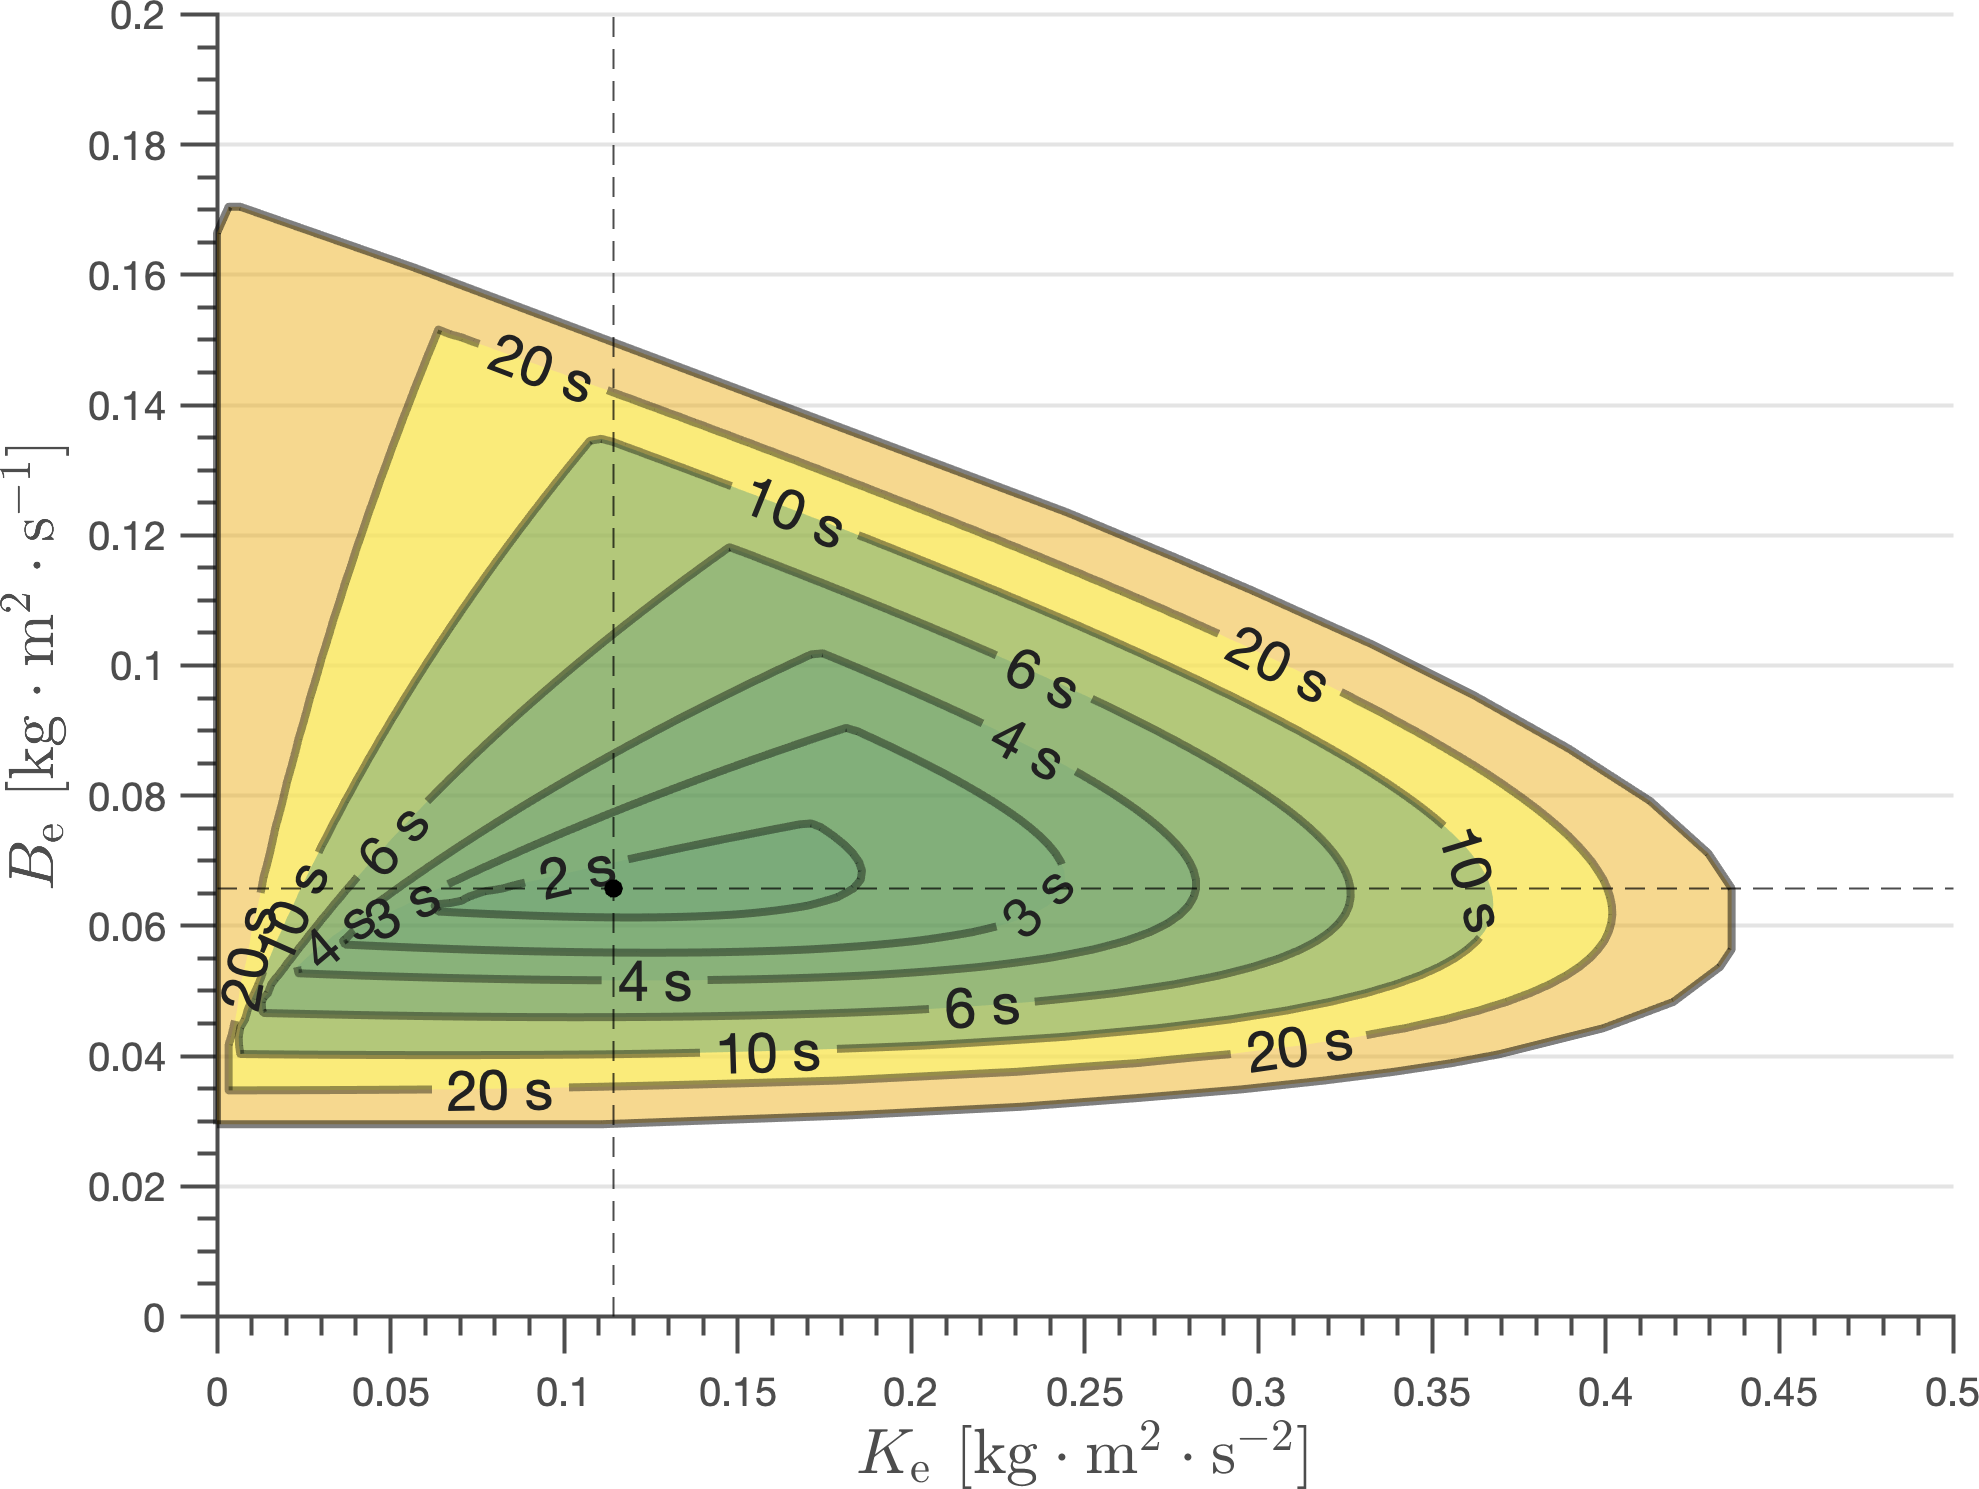
\includegraphics[width=\textwidth]{images/time_delay_stab_map_discrete.png}
    \caption{Diszkrét idejű stabilitástérkép}\label{fig:time_delay_stab_map_discrete}
    \end{center}
\end{figure}
A kontúrok a különböző becsült beállási időket jelölnek, melyek a legnagyobb abszolút értékű sajátérték 
alapján lettek meghatározva:
\begin{align}
    \begin{split}
        t_\RM s \approx \tau_\RM d \frac{\ln{0.02}}{\ln{|\lambda|_\RM{max}}}
    \end{split}        
\end{align}
alapján, ahol \(\tau_\RM d\) a mintavételezési idő és \(|\lambda|_\RM{max}\) jelöli a legnagyobb sajátértéket 
abszolút értékben. Az alkalmazott paraméterekkel a minimális beállási idő közelítőleg 1.2 s. 

A diszkretizáció negatív hatással van a rendszer stabilitására. A folytonos idejű időkéséses rendszernél 0.1 s 
időkéséssel még mindig végtelen nagy a stabil régió ugyanezen paraméterekkel. Az impedancia modell által 
előírt beállási időt összehasonlítva a becsült beállási idővel ábrázolja a~\ref{fig:time_delay_stab_map_discrete_diff}.
ábra.

\begin{figure}[H]
    \begin{center}
    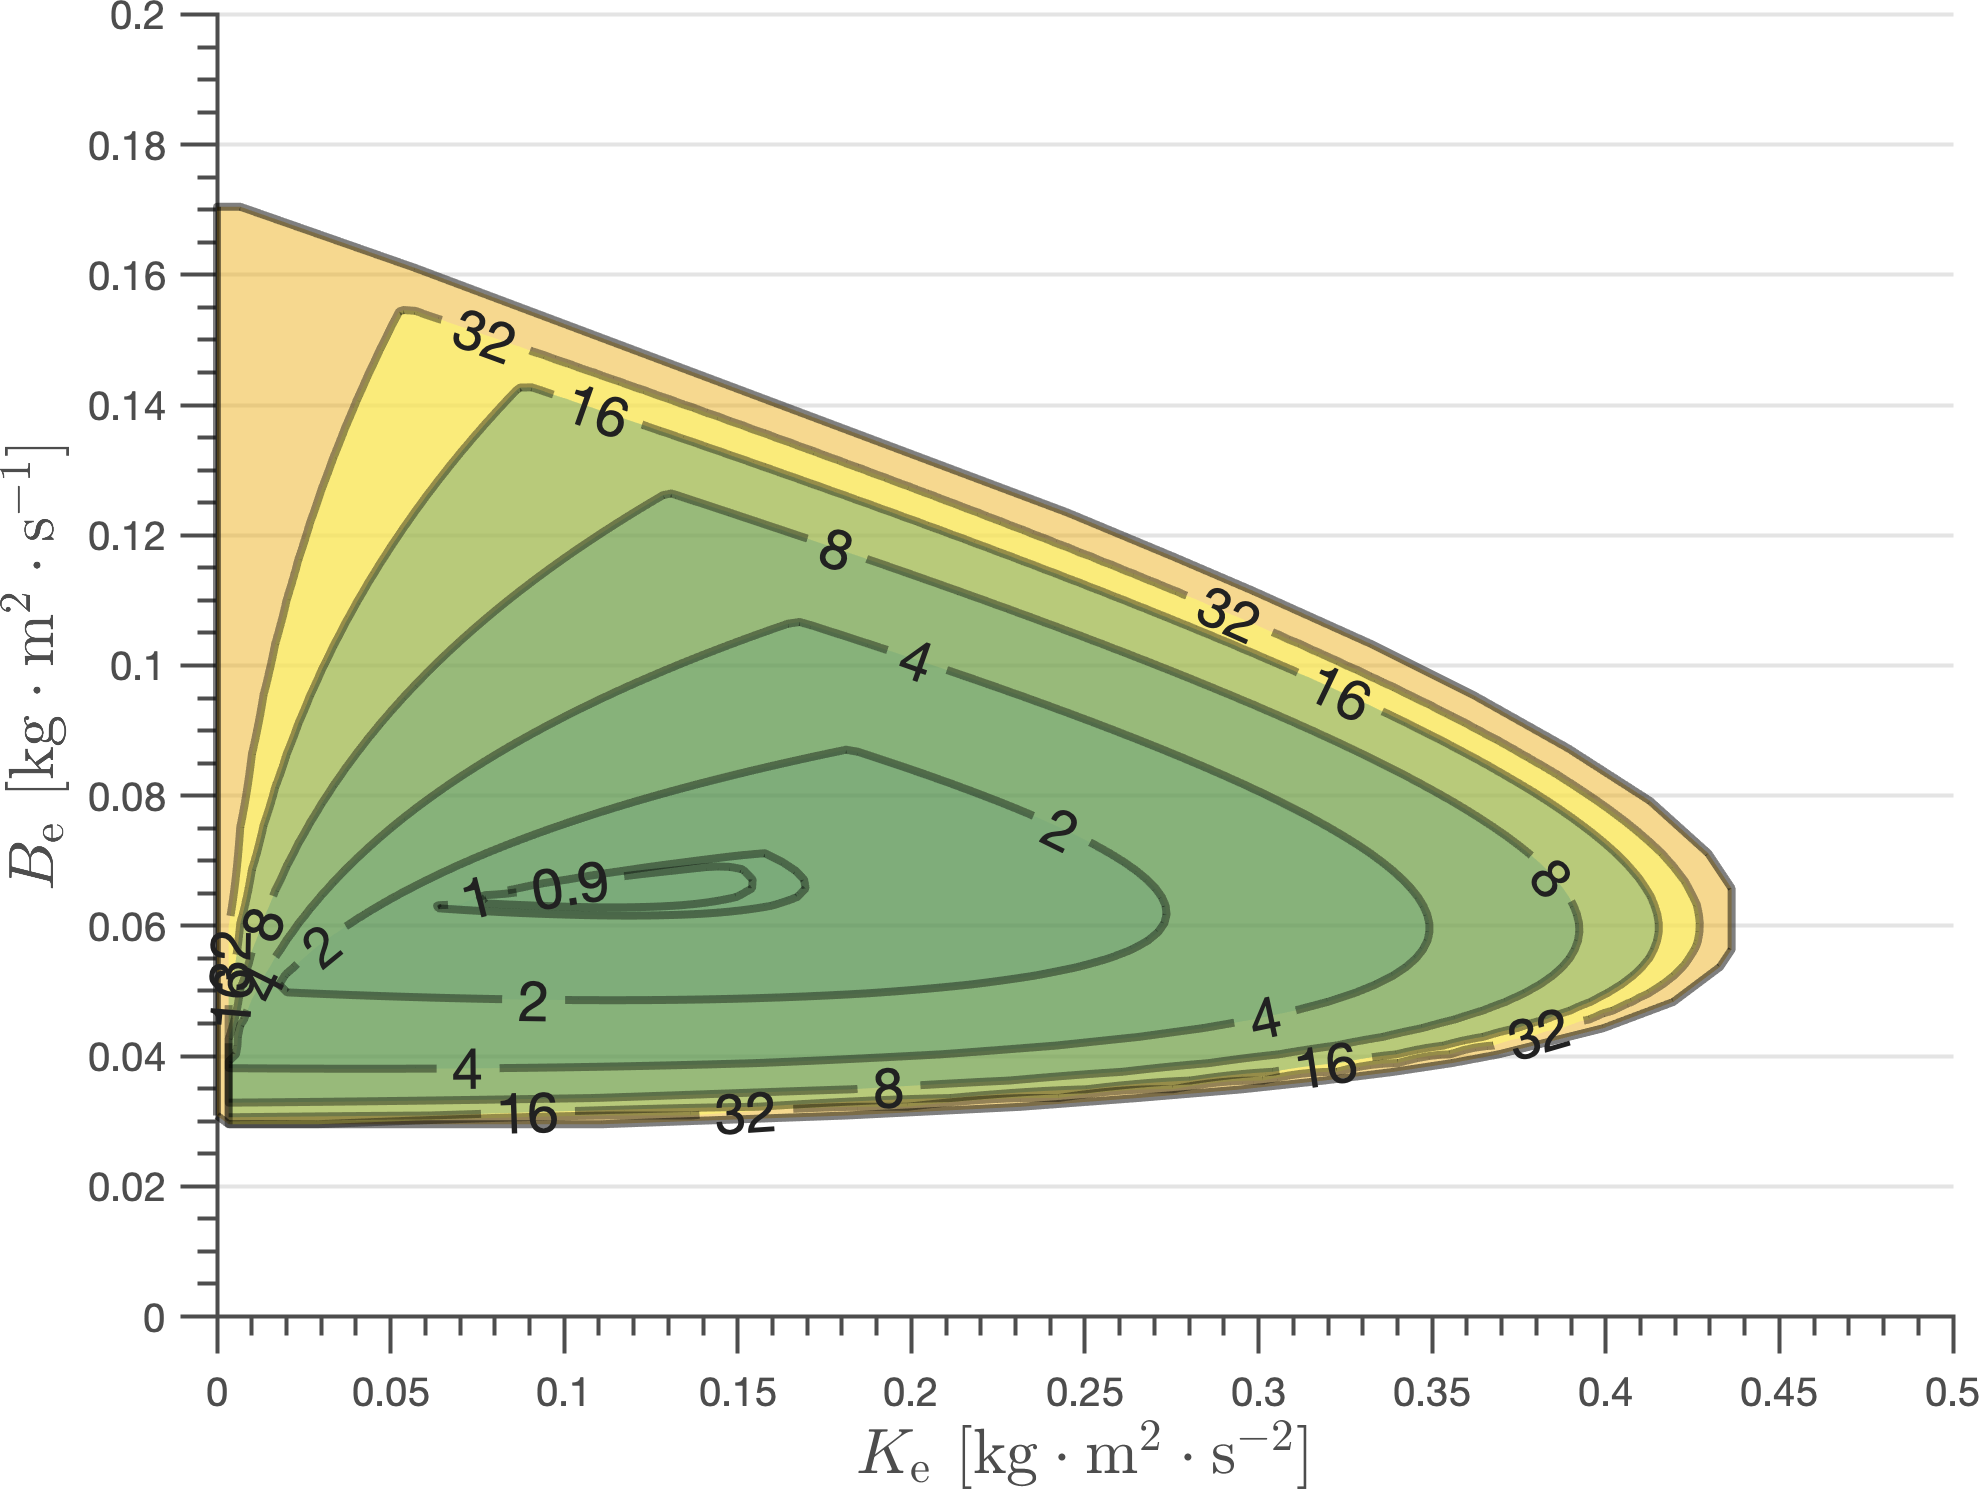
\includegraphics[width=\textwidth]{images/time_delay_stab_map_discrete_diff.png}
    \caption{Diszkrét idejű stabilitástérkép}\label{fig:time_delay_stab_map_discrete_diff}
    \end{center}
\end{figure}

A kontúrok a becsült és az előírt beállási idők hányadosát jelölik. Az alkalmazás specifikációjától függően lehet, 
hogy csak egy igen kis része felhasználható a stabil tartomáynak. Az ábrán megfigyelhető, hogy van olyan tartomány is, 
ahol az előírtnál gyorsabban beáll a rendszer.

A stabilitási határon legalább egy sajátérték abszolút értékben egy. Ennek következtében a rendszer 
\(t\rightarrow\infty\) határértékben csillapítatlan rezgőmozgást végez. A rezgőmozgás frekvenciája és az 
impedancia modell paraméterei közötti összefüggés numerikusan meghatározható például a diszkrét 
Fourier-transzformáció segítségével. A legnagyobb frekvencia a mintavételezési frekvencia fele a Nyquist--Shannon 
mintavételezési tétel alapján 
\begin{align}
    f_\RM{max} = \frac{1}{2\tau_\RM d}\,.
\end{align}

A frekvencia felbontás pedig a mintavételek száma és a mintavételezési frekvencia alapján
\begin{align}
    \Delta f = \frac{1}{N\tau_\RM d}\,.
\end{align}

A stabil tartomány jobb széle \(B_\RM e\) értékével lett paraméterezve. Ezután minden pontban  
\(N = 100\) időlépésen át lett szimulálva a rendszer. A diszkrét Fourier-transzformált 
legnagyobb abszolút értékű frekvenciája és \(B_\RM e\) közötti kapcsolat látható 
a~\ref{fig:time_delay_stab_map_discrete_fourier}. ábra jobb oldali grafikonján. A vízszintes 
tengelyre a csillapítatlan rezgési frenvencia és a mintavételezési frekvencia hányadosa került.
\begin{figure}[H]
    \begin{center}
    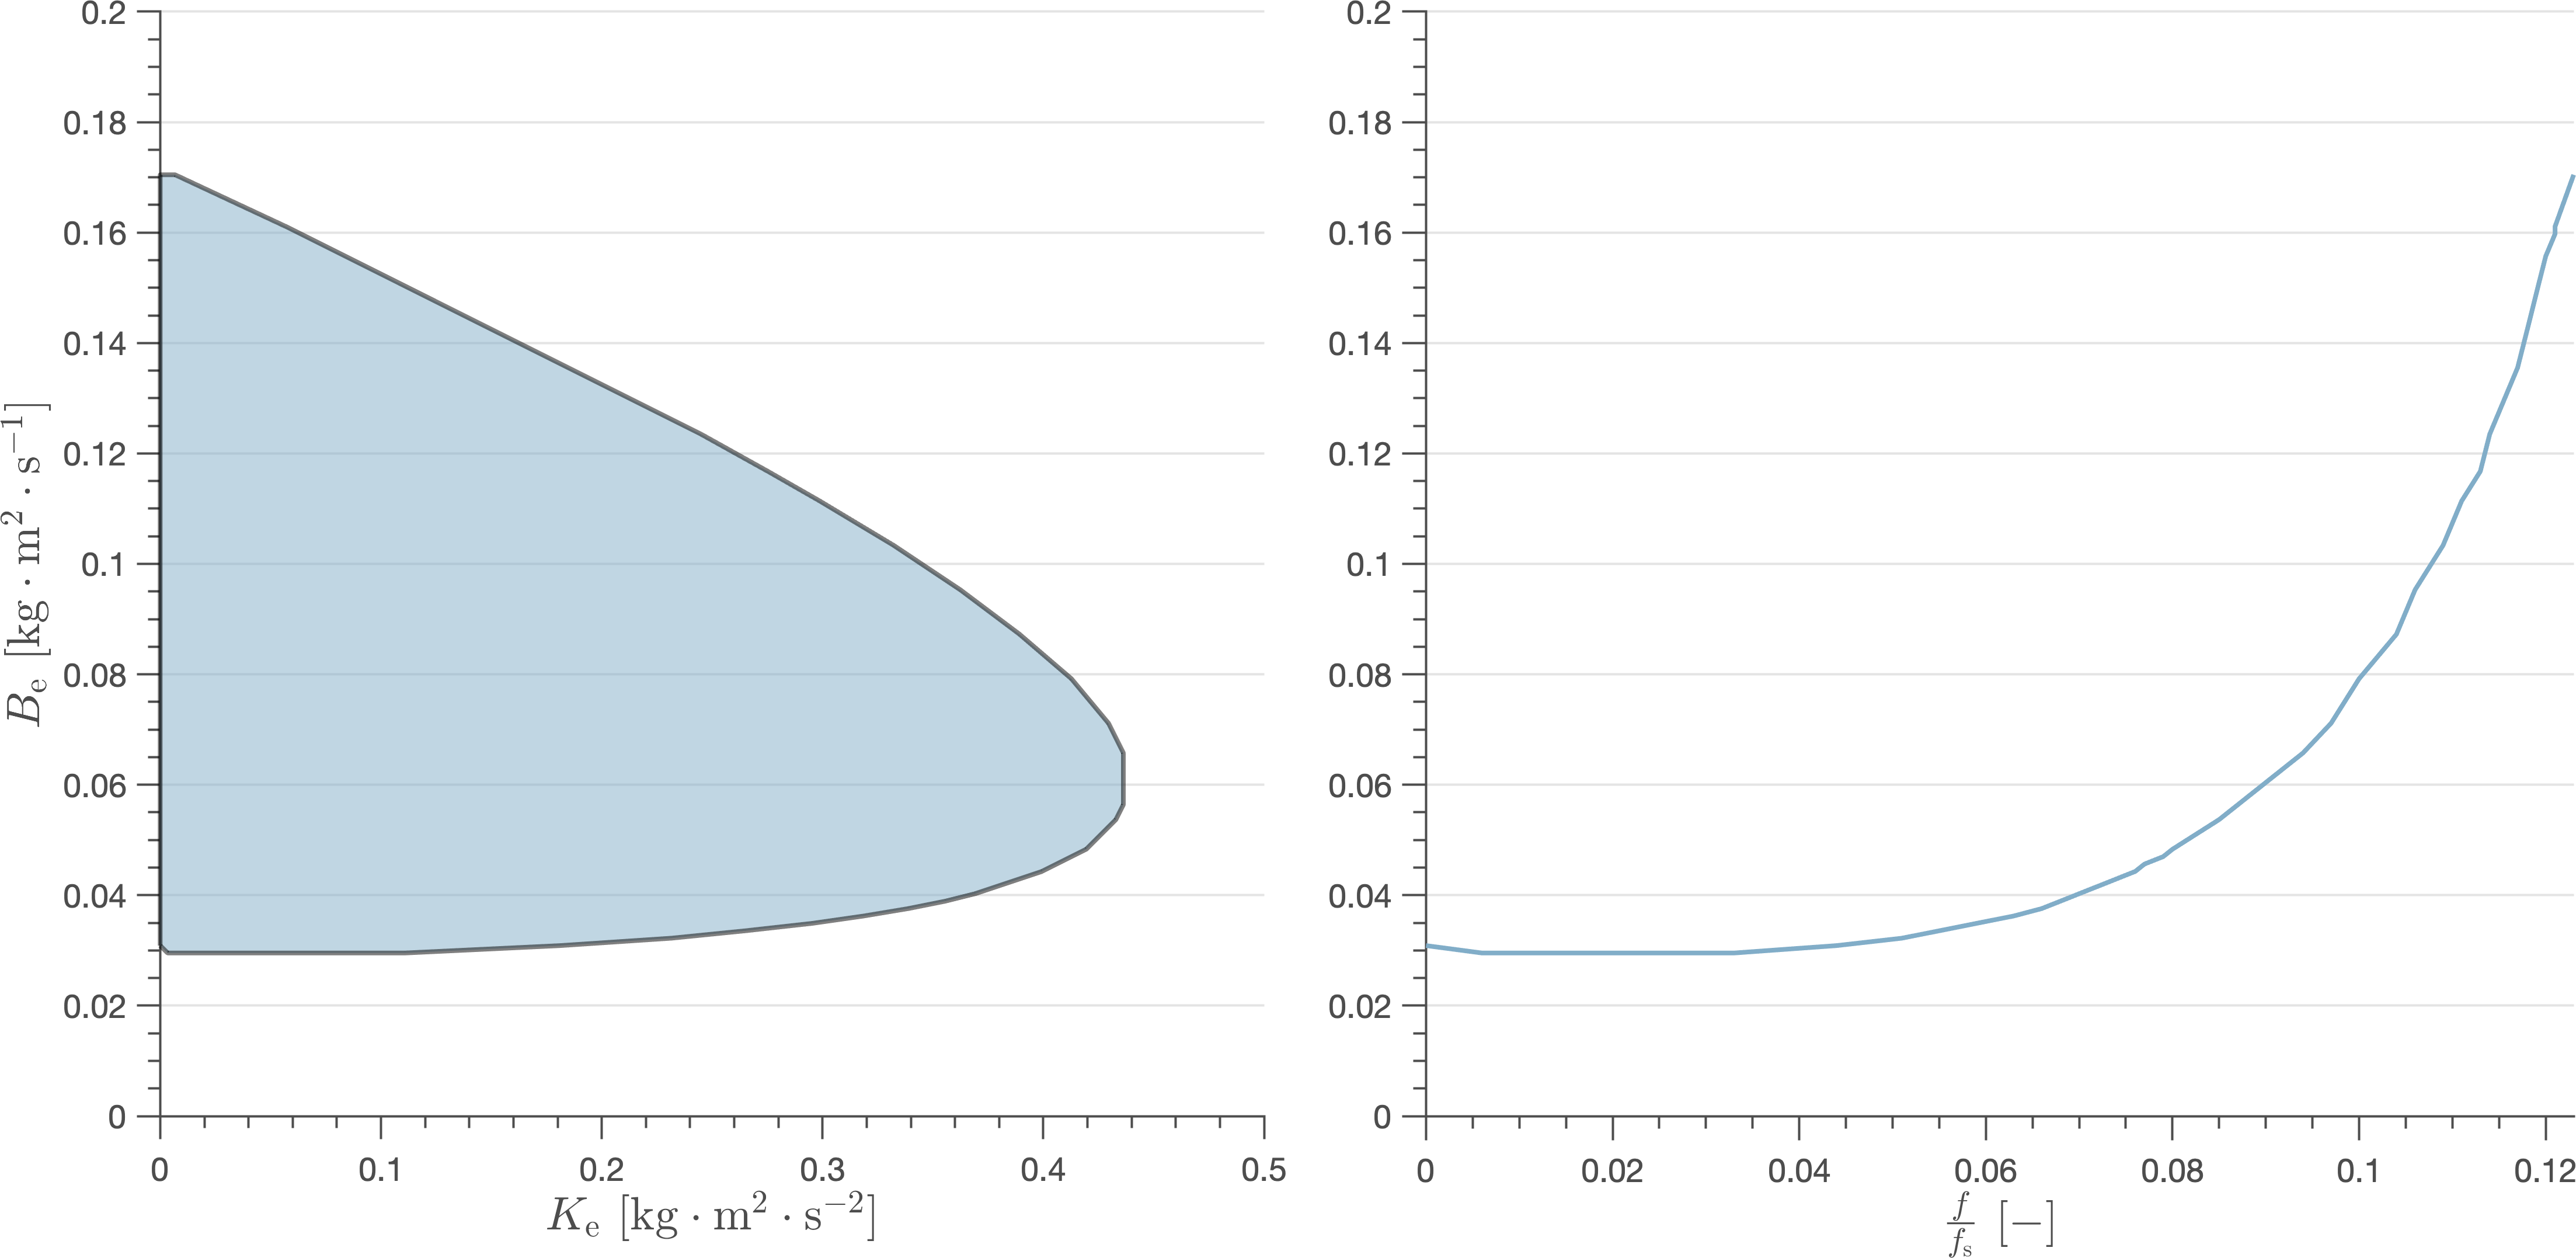
\includegraphics[width=\textwidth]{images/time_delay_stab_map_discrete_fourier.png}
    \caption{Diszkrét idejű stabilitástérkép}\label{fig:time_delay_stab_map_discrete_fourier}
    \end{center}
\end{figure}
A stabil tartomány bal alsó sarkában nullától indulva egyre nő a csillapítatlan 
rezgési frekvencia, mig a tartomány bal felső sarkában el nem éri a maximumát, mely ebben az 
esetben \(\approx 1.2~\RM{Hz}\)
